\documentclass[10pt,a4paper]{article}

\usepackage[utf8]{inputenc}
\usepackage{cmap}
\usepackage[T1]{fontenc}
\usepackage[scaled=0.95]{helvet}
\renewcommand{\familydefault}{\sfdefault}
\usepackage[english]{babel}
\usepackage[a4paper,margin=1.55cm]{geometry}
\usepackage{graphicx}
\usepackage{xcolor}
\usepackage{enumitem}
\usepackage{needspace}
\usepackage[colorlinks=true,urlcolor=accent,linkcolor=accent,citecolor=accent]{hyperref}

\definecolor{navy}{HTML}{16344A}
\definecolor{accent}{HTML}{16877A}
\definecolor{pale}{HTML}{EDF4F3}
\definecolor{muted}{HTML}{5C6B73}

\setlength{\parindent}{0pt}
\setlength{\parskip}{1pt}
\setlist[itemize]{label={\large\textbullet},leftmargin=1.35em,itemsep=1pt,topsep=2pt}
\urlstyle{same}

\newcommand{\cvsection}[1]{%
    \vspace{11pt}%
    {\large\bfseries\color{navy}#1}\par
    \vspace{2pt}{\color{accent}\rule{\linewidth}{1.2pt}}\par
    \vspace{5pt}%
}

\begin{document}

\noindent
\colorbox{navy}{%
    \begin{minipage}{\dimexpr\textwidth-2\fboxsep\relax}
        \color{white}
        \begin{minipage}[c]{0.72\linewidth}
            {\fontsize{18}{21}\selectfont\bfseries CARLOS ALEJANDRO FREITAS TEIXEIRA}\par
            \vspace{3pt}
            {\large\bfseries\color{pale}Systems Engineer | Master's in Artificial Intelligence}\par
            \vspace{7pt}
            {\small Porto, Portugal \textbar{} Email: \href{mailto:carlosfreitasingsistemas@gmail.com}{\textcolor{white}{carlosfreitasingsistemas@gmail.com}} \textbar{} +351 937797609\par}
            \vspace{3pt}
            {\small
                \href{https://github.com/CarlosFreitasING}{\textcolor{white}{GitHub}}
                \textcolor{pale}{\textbar{}}
                \href{https://www.linkedin.com/in/carlos-alejandro-freitas-teixeira-82921a249/}{\textcolor{white}{LinkedIn}}
                \textcolor{pale}{\textbar{}}
                \href{https://carlosfreitas32.wixsite.com/portafolio}{\textcolor{white}{Portfolio}}
            }
        \end{minipage}
        \hfill
        \begin{minipage}[c]{0.22\linewidth}
            \centering
            \fcolorbox{white}{pale}{%
                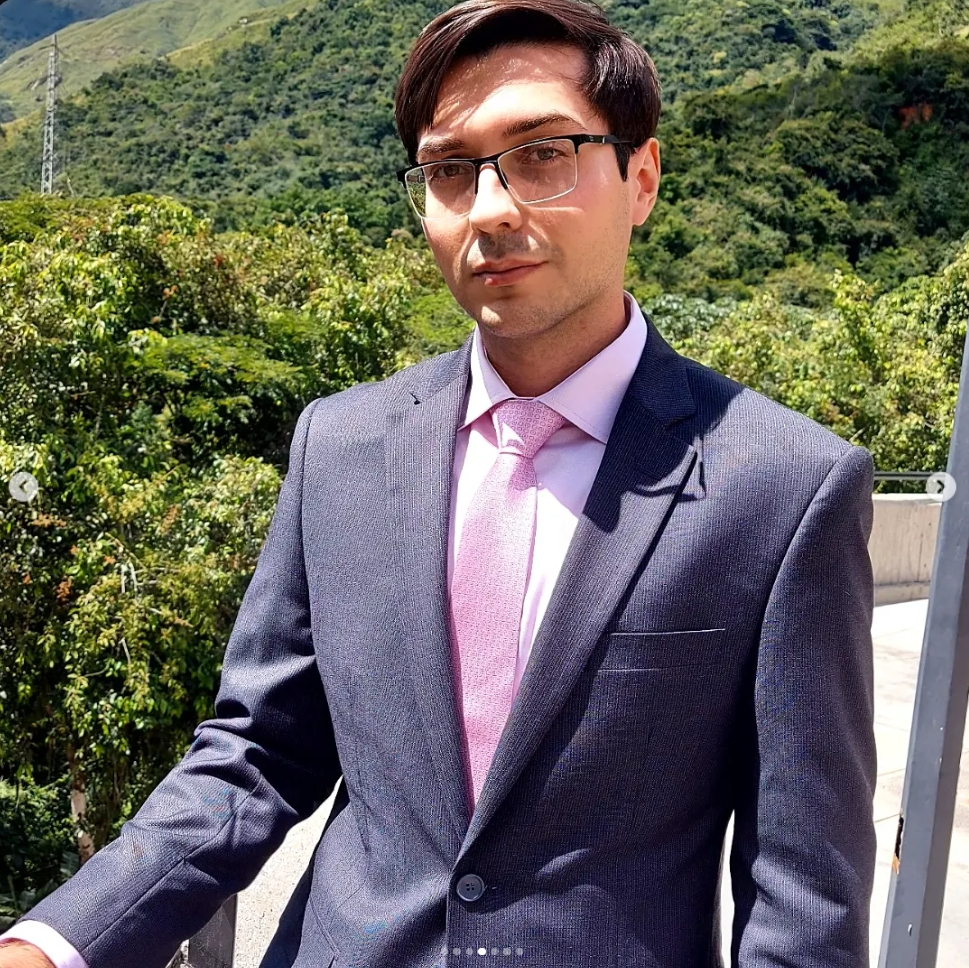
\includegraphics[width=3.2cm,height=3.2cm,keepaspectratio,trim=6cm 12cm 6cm 0cm,clip]{assets/foto.jpeg}%
            }
        \end{minipage}
    \end{minipage}%
}

\cvsection{PROFILE}
\colorbox{pale}{%
    \parbox{\dimexpr\textwidth-2\fboxsep\relax}{%
        Systems Engineer and Master's graduate in Artificial Intelligence with experience in applied R\&D of AI-based solutions. I have strong knowledge of Computer Vision, Machine/Deep Learning, LLMs, Edge AI, and Robotics (ROS 2), complemented by hands-on full-stack development experience. Focused on designing scalable architectures, implementing on-device inference models, and deploying user-oriented technological solutions in real-world environments.
    }%
}

\cvsection{EXPERIENCE}

\Needspace{4\baselineskip}
\textbf{\large Artificial Intelligence Researcher and Developer (R\&D)}\\
{\color{muted}GECAD - ISEP \textbar{} Porto, Portugal}

\vspace{4pt}
\textbf{\color{accent}CRIARTE Project \textbar{} Oct 2025 -- Present}\\
I contribute to a European innovation project that aims to transform the construction industry through AI, robotics, and emerging technologies as part of Industry 5.0.
\begin{itemize}
    \item I research, train, and evaluate Machine Learning models and clustering algorithms to analyse wearable-sensor data and identify patterns associated with workers' physiological states.
    \item I fine-tune YOLO models to detect people and estimate human poses using computer vision systems.
    \item I develop distributed architectures based on ROS 2 to integrate computer vision and physiological monitoring systems.
    \item \textbf{Technology Stack:} ROS 2, YOLO, ReID, Computer Vision, Machine Learning, GMM, AHC, Python, C++.
\end{itemize}

\vspace{2pt}
\textbf{\color{accent}WAI Project (Wellbeing@Artificial Intelligence) \textbar{} Nov 2025 -- Jun 2026}\\
I contributed to a European research initiative using AI solutions to promote student wellbeing and support anxiety management and mental health.
\begin{itemize}
    \item I developed and published the ``WellBe'' mobile app for \href{https://play.google.com/store/apps/details?id=com.caloale.waiv1\&hl=en_US}{Android} and \href{https://apps.apple.com/ie/app/wellbe-journaling-app/id6758772082}{iOS}.
    \item I achieved international deployment, reaching users in 7 countries and more than 200 downloads.
    \item I implemented AI models with on-device inference through an offline-first architecture to protect user privacy.
    \item \textbf{Technology Stack:} React Native, Expo, EAS Build, SQLite, ONNX Runtime, TinyBERT.
\end{itemize}

\Needspace{4\baselineskip}
\textbf{\large Freelance Software Developer}\\
{\color{muted}Remote \textbar{} Oct 2022 -- Present}
\begin{itemize}
    \item I design and develop full-stack solutions for clients and businesses, digitalising and automating processes.
    \item I develop web platforms and management systems, including a digital loyalty application for a restaurant business (See: \href{https://avenidakebab.com/}{Loyalty Website}).
    \item I design databases, configure user authentication and permission management, and integrate services through APIs.
    \item \textbf{Technology Stack:} Angular, React, PWA, iOS/Android, SQL, RLS, APIs, and microservices.
\end{itemize}

\Needspace{4\baselineskip}
\textbf{\large Junior Full-Stack Developer and Analyst}\\
{\color{muted}INFOCENT C.A. \textbar{} Caracas, Venezuela \textbar{} Oct 2023 -- Sep 2024}
\begin{itemize}
    \item I contributed to the modernization of a legacy payroll management application for enterprise clients.
    \item I developed and implemented new frontend and backend features for the payroll system.
    \item I performed corrective maintenance, resolved incidents, and optimized system features.
    \item \textbf{Technology Stack:} Angular, Spring Boot, Java, SQL, relational databases.
\end{itemize}

\Needspace{14\baselineskip}
\textbf{\large Software Developer and Digital Transformation Designer}\\
{\color{muted}Universidad Metropolitana (UNIMET) \textbar{} Caracas, Venezuela \textbar{} 2021 -- 2022}
\begin{itemize}
    \item I led the digital transformation and automated the academic request system, eliminating administrative bottlenecks, streamlining workflows, and removing manual request processing.
    \item I designed and developed a full-stack interactive web platform for student self-service, with real-time notifications and an administration panel.
    \item I deployed the software to production and achieved sustained adoption by the university community. The platform has been in use since 2022 (See: \href{https://script.google.com/macros/s/AKfycbw3h26r_mjt0jow79RT9dnPaUKZ81dVUsF8qDeEjp7wsRg-ldqHjlB9L0FJYP_Uc_LXUw/exec}{Study Control Web Portal}).
    \item \textbf{Technology Stack:} Google Apps Script, JavaScript, HTML/CSS, Google Sheets, SQL.
\end{itemize}

\cvsection{EDUCATION}
\textbf{Master's in Artificial Intelligence \textbar{} Instituto Superior de Engenharia do Porto (ISEP)}\\
{\color{muted}Porto, Portugal \textbar{} 2024 -- Oct 2026 (completed)}\\
Master's thesis: ``Análise e Previsão do Estado Fisiológico de Trabalhadores em Obra através de Gémeos Digitais Humanos e Aprendizagem Automática'' (\href{https://drive.google.com/file/d/1xlqiDRtNX2Xj5_9TnHy6inUlAnseSHbF/view?usp=drive\_link}{thesis PDF}).

\vspace{5pt}
\textbf{Systems Engineering \textbar{} Universidad Metropolitana (UNIMET)}\\
{\color{muted}Caracas, Venezuela \textbar{} 2016 -- 2022}\\
Bachelor's thesis: ``Web application for managing and tracking academic document requests at Universidad Metropolitana'' (\href{https://unimet.ent.sirsi.net/client/es_ES/default/search/detailnonmodal/ent:\%24002f\%24002fSD\_ILS\%24002f0\%24002fSD\_ILS:132264/one}{UNIMET catalogue record}).

\cvsection{PUBLICATIONS \& CONFERENCES}
\begin{itemize}
    \item \textbf{Article:} ``A Review of Physiological Monitoring and Prediction in Workers in High-Risk Construction Environments'', presented at INISTA 2026 (Guimarães, Portugal, 17--19 September 2026). Links: \href{https://inista2026.di.uminho.pt/pdf/INISTA\_Official\_Program.pdf}{official programme} | \href{https://drive.google.com/file/d/1Kh2M0t4dUh3F5vFrKY5sZMfaRxV1H2PT/view?usp=sharing}{article PDF}.
    \item \textbf{Invited speaker:} ``Artificial Intelligence in Health and Mental Health: Challenges, Opportunities and Future Perspectives'', at the final dissemination event of the Erasmus+ project WELLBEING@ARTIFICIAL INTELLIGENCE (ISEP, Porto, Portugal, 9--10 July 2026).
\end{itemize}

\cvsection{TECHNICAL SKILLS}
\begin{itemize}
    \item \textbf{Artificial Intelligence \& Data:} Computer Vision, Pose Estimation (YOLO), ReID, NLP, LLMs, Fine-tuning, Edge AI, ONNX Runtime, PyTorch, OpenCV, Machine Learning (ANN, CNN, RNN), Clustering (GMM/AHC).
    \item \textbf{Programming Languages:} Python, TypeScript, JavaScript, Java, C++, C\#, HTML/CSS.
    \item \textbf{Development \& Architecture:} React Native, Angular, Spring Boot, ASP.NET, Flutter, Offline-first / Local-first architectures, Serverless, ROS 2, PWA.
    \item \textbf{Databases \& Tools:} PostgreSQL, Supabase, SQLite, MySQL, MongoDB, SQL Server, Firebase, Git.
\end{itemize}

\cvsection{CERTIFICATIONS}
C1 English Certificate and Conversational English Certificate \textbar{} Fyr Lois \textbar{} 2019 -- 2022.

\vspace{4pt}
Certificates of Competency \textbar{} Universidad Metropolitana \textbar{} 2022
\begin{itemize}
    \item Information Systems Analyst.
    \item Data Design and Processing Analyst.
    \item Basic Operations Research Assistant Engineer.
    \item Network Analyst.
\end{itemize}

\cvsection{LANGUAGES}
\textbf{Spanish:} native \hfill
\textbf{English:} C1 \hfill
\textbf{Portuguese:} conversational

\end{document}
